%# -*- coding: utf-8-unix -*-
%%==================================================
%% chapter01.tex for SJTU Master Thesis
%%==================================================

\chapter{绪论}
\label{chap:introduction}

\section{引言}
\label{sec:objective}
隐私是一种与公共、群体利益无关,不便或者不愿他人知道的、应予以保密的信息,是不以他人是否承认或评价为转移的存在。从人类有意识开始,隐私意识便是最先表现出来的本能特征,伴随着时代文明的发展,人类具有越来越强的隐私保护意识。“数据时代”的飞速发展使得信息数据的采集、存储和发布变得更加方便快捷,海量数据的处理技术以及数据挖掘、机器学习算法的应用使得数据的共享和分析变得更加高效准确,与此同时新的隐私攻击手段,黑客技术也在不断涌现。可见科技和时代的发展在带给我们高品质生活的同时,数据中的隐私保护问题面临着愈加严峻的挑战。
本课题基于最高隐私保障的差分隐私技术,通过设计对高纬度查询问题具有良好扩展性的非交互式差分隐私匿名算法,有效提升了发布数据在后续数据挖掘分类算法中的分类准确度。本章节将简要介绍相关的课题背景知识,总结各类隐私保护算法和面向数据挖掘分类问题的研究现状,最后明确研究目标和所要解决的问题。


\section{课题研究背景}

\subsection{隐私及隐私保护}  %隐私的定义,度量,泄露风险及隐私保护研究方向

隐私指的是个体不愿被外界获悉的敏感属性,比如个人的病理特征,资产状况,家庭住址等。隐私分为两类\cite{Defining Privacy for Data}:(1)个人隐私(individual privacy):任何可以直接或间接标识特定人物且不愿被披露的信息,可以是个人的物理信息,生理信息或社会属性信息等。(2)共同隐私(corporate privacy):包含了所有人共同的个人隐私的信息,如工厂工人的薪资分布。

隐私的保护程度可以用隐私的“披露风险”(disclosure risk)\cite{l-diversity}来度量,披露风险越高意味着隐私保护程度越低。披露风险是与攻击者所具备的背景知识(background knowledge)相关的\cite{面向数据库应用的隐私保护研究综述},若s表示隐私信息,Pr[E]表示事件E发生的概率,那么在公布背景知识E的前提下隐私信息s披露的风险\textsc{R}(s,E)表示为
\[
	\textsc{R}(s,E) = Pr(E_{s}).
\]
披露风险\textsc{R}(s,E)可以用来度量隐私保护程度,如$l$-diversity算法\cite{l-diversity}保证隐私披露风险不超过1/$l$,$m$-Invariance算法\cite{m-Invariance}的披露风险不超过1/$m$。

隐私保护的研究方向是由具体应用领域的需求来决定。面向数据挖掘类应用的隐私保护技术主要是研究针对某类数据挖掘算法,根据其特性设计出适应性良好的隐私保护算法,如Clustering\cite{clustering}算法;基于数据发布的隐私保护技术,主要是通过泛化或加密技术发布处理后的数据提供给各类应用,如一系列匿名化算法\cite{multidimensional k anonymity};面向分布式环境下的隐私保护技术,如在智能电网中的应用\cite{Distributed Privacy}。

隐私保护手段大体上分为4类\cite{面向数据库应用的隐私保护研究综述}:(1)基于数据失真(distorting)的技术,如通过添加噪音(noise)的方式达到模糊敏感数据的目的,同时保持数据集的统计特征。(2)基于数据加密技术隐藏敏感数据。(3)基于限制发布的保护技术,如泛化数据域。(4)结合以上三种方式的优点生成的新方法。


\subsection{差分隐私背景} %交互和非交互框架,隐私代价分配和消耗 列联表 直方图

差分隐私不同于传统的隐私保护技术,它对隐私披露风险给出了严谨的量化证明,并且定义了严格的攻击模式,因此不关心攻击者所获取的背景知识。通过拉普拉斯加噪机制\cite{Dwork Calibrating}设计满足差分隐私定义的算法,就能够给数据提供最高级别的隐私保障力度。差分隐私技术的研究主要在于两个方面:(1)如何设计满足差分隐私定义的隐私保护算法。(2)如何减少噪音扰动,保证加噪后数据的高可用性。

差分隐私保护框架分为两种:交互式框架和非交互式框架,如下图\ref{fig:interactive framework}和图\ref{fig:non-interactive framework}所示。在交互式框架中,用户提交查询请求给数据库之后,数据库的应答作为某种差分隐私处理算法的输入,返回输出结果给用户。这个过程中差分隐私处理算法成为了用户和数据库之间的查询接口,但经过一定数量的查询之后耗尽隐私预算$\varepsilon$,对于之后的查询就无法保证隐私保护质量了,因此不再满足差分隐私定义。
在非交互式框架中,数据库先将包含隐私信息的原数据集交于差分隐私算法处理,接着发布整个处理后数据集给用户,或者采用常规数据库查询模式给予应答。这个离线模式的框架具有诸多优点,并且不存在隐私预算耗尽的问题,更多的研究点在于考虑如何提升发布数据可用性和分析准确度。

\begin{figure}[!htp]
	\centering
	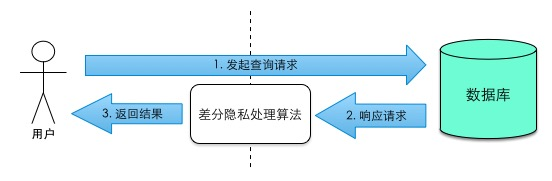
\includegraphics[width=5in]{chap1/interactive}
	\bicaption[fig:interactive framework]{图}{交互式框架}{Fig.}{interactive framework}
\end{figure}

\begin{figure}[!htp]
	\centering
	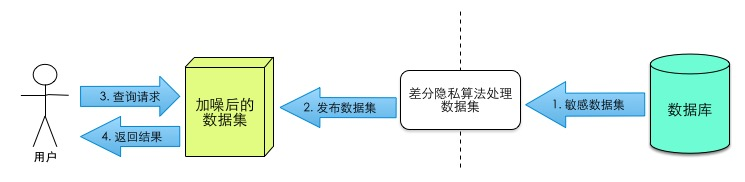
\includegraphics[width=5in]{chap1/non-interactive}
	\bicaption[fig:non-interactive framework]{图}{非交互式框架}{Fig.}{non-interactive framework}
\end{figure}



\subsection{匿名化算法}  %k匿名算法

\subsection{决策树} %主要的数据挖掘分类算法,信息增益,C4.5,CART对于离散和连续属性的处理问题

